\documentclass{extbook}[14pt]
\usepackage{multicol, enumerate, enumitem, hyperref, color, soul, setspace, parskip, fancyhdr, amssymb, amsthm, amsmath, latexsym, units, mathtools}
\everymath{\displaystyle}
\usepackage[headsep=0.5cm,headheight=0cm, left=1 in,right= 1 in,top= 1 in,bottom= 1 in]{geometry}
\usepackage{dashrule}  % Package to use the command below to create lines between items
\newcommand{\litem}[1]{\item #1

\rule{\textwidth}{0.4pt}}
\pagestyle{fancy}
\lhead{}
\chead{Answer Key for Module6 Version B}
\rhead{}
\lfoot{7334-5530}
\cfoot{}
\rfoot{test}
\begin{document}
\textbf{This key should allow you to understand why you choose the option you did (beyond just getting a question right or wrong). \href{https://xronos.clas.ufl.edu/mac1105spring2020/courseDescriptionAndMisc/Exams/LearningFromResults}{More instructions on how to use this key can be found here}.}

\textbf{If you have a suggestion to make the keys better, \href{https://forms.gle/CZkbZmPbC9XALEE88}{please fill out the short survey here}.}

\textit{Note: This key is auto-generated and may contain issues and/or errors. The keys are reviewed after each exam to ensure grading is done accurately. If there are issues (like duplicate options), they are noted in the offline gradebook. The keys are a work-in-progress to give students as many resources to improve as possible.}

\rule{\textwidth}{0.4pt}

\begin{enumerate}\litem{
Describe the zero behavior of the zero $x = -2$ of the polynomial below.
\[ f(x) = 6(x - 5)^{7}(x + 5)^{4}(x + 2)^{9}(x - 2)^{6} \]The solution is the graph below.
    \begin{center}
        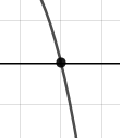
\includegraphics[width=0.3\textwidth]{../Figures/polyZeroBehaviorAB.png}
    \end{center}

\textbf{General Comment:} You will need to sketch the entire graph, then zoom in on the zero the question asks about.
}
\litem{
Write an equation that \textit{could} represent the graph below.

\begin{center}
    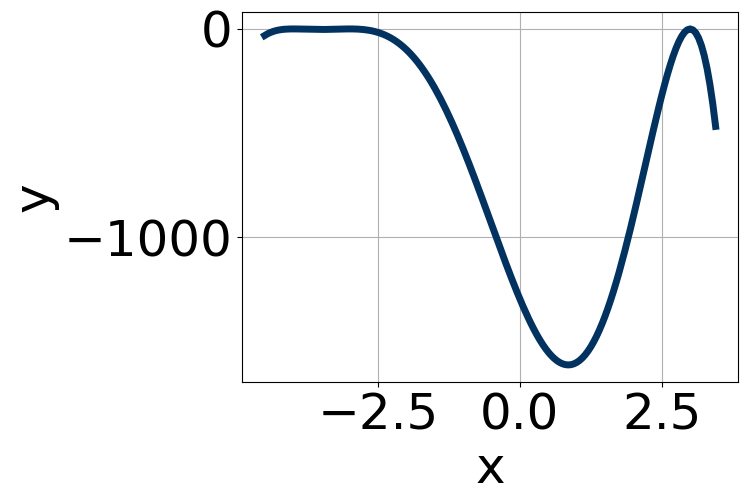
\includegraphics[width=0.5\textwidth]{../Figures/polyGraphToFunctionB.png}
\end{center}


The solution is \( -19(x + 3)^{4} (x + 4)^{10} (x - 3)^{8} \).\begin{enumerate}[label=\Alph*.]
\textbf{Plausible alternative answers include:}* This is the correct option.
The factor $(x - 3)$ should have an even power and the leading coefficient should be the opposite sign.
This corresponds to the leading coefficient being the opposite value than it should be.
The factors $(x + 4)$ and $(x - 3)$ should both have even powers.
The factor $(x - 3)$ should have an even power.
\end{enumerate}

\textbf{General Comment:} General Comments: Draw the x-axis to determine which zeros are touching (and so have even multiplicity) or cross (and have odd multiplicity).
}
\litem{
Construct the lowest-degree polynomial given the zeros below.
\[ \frac{-4}{3}, \frac{-5}{3}, \text{ and } -7 \]The solution is \( 9x^{3} +90 x^{2} +209 x + 140 \).\begin{enumerate}[label=\Alph*.]
\textbf{Plausible alternative answers include:}$9x^{3} +66 x^{2} +x -140$, which corresponds to multiplying out $(3x -4)(3x + 5)(x + 7)$.
$9x^{3} -90 x^{2} +209 x -140$, which corresponds to multiplying out $(3x -4)(3x -5)(x -7)$.
* $9x^{3} +90 x^{2} +209 x + 140$, which is the correct option.
$9x^{3} +36 x^{2} -169 x + 140$, which corresponds to multiplying out $(3x -4)(3x -5)(x + 7)$.
$9x^{3} +90 x^{2} +209 x -140$, which corresponds to multiplying everything correctly except the constant term.
\end{enumerate}

\textbf{General Comment:} To construct the lowest-degree polynomial, you want to multiply out $(3x + 4)(3x + 5)(x + 7)$
}
\litem{
Describe the zero behavior of the zero $x = -8$ of the polynomial below.
\[ f(x) = -6(x + 2)^{11}(x - 2)^{7}(x + 8)^{3}(x - 8)^{2} \]The solution is the graph below.
    \begin{center}
        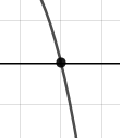
\includegraphics[width=0.3\textwidth]{../Figures/polyZeroBehaviorCopyAB.png}
    \end{center}

\textbf{General Comment:} You will need to sketch the entire graph, then zoom in on the zero the question asks about.
}
\litem{
Construct the lowest-degree polynomial given the zeros below.
\[ \frac{1}{2}, \frac{3}{4}, \text{ and } 4 \]The solution is \( 8x^{3} -42 x^{2} +43 x -12 \).\begin{enumerate}[label=\Alph*.]
\textbf{Plausible alternative answers include:}$8x^{3} -34 x^{2} +5 x + 12$, which corresponds to multiplying out $(2x + 1)(4x -3)(x -4)$.
$8x^{3} -22 x^{2} -37 x -12$, which corresponds to multiplying out $(2x + 1)(4x + 3)(x -4)$.
* $8x^{3} -42 x^{2} +43 x -12$, which is the correct option.
$8x^{3} -42 x^{2} +43 x + 12$, which corresponds to multiplying everything correctly except the constant term.
$8x^{3} +42 x^{2} +43 x + 12$, which corresponds to multiplying out $(2x + 1)(4x + 3)(x + 4)$.
\end{enumerate}

\textbf{General Comment:} To construct the lowest-degree polynomial, you want to multiply out $(2x -1)(4x -3)(x -4)$
}
\litem{
Describe the end behavior of the polynomial below.
\[ f(x) = 2(x + 7)^{4}(x - 7)^{9}(x - 4)^{2}(x + 4)^{2} \]The solution is the graph below.
    \begin{center}
        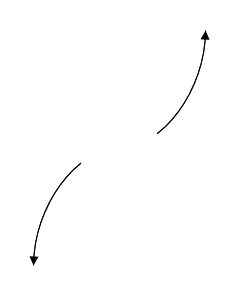
\includegraphics[width=0.3\textwidth]{../Figures/polyEndBehaviorCopyDB.png}
    \end{center}

\textbf{General Comment:} Remember that end behavior is determined by the leading coefficient AND whether the \textbf{sum} of the multiplicities is positive or negative.
}
\litem{
Construct the lowest-degree polynomial given the zeros below.
\[ -2 + 2 i \text{ and } -2 \]The solution is \( x^{3} +6 x^{2} +16 x + 16 \).\begin{enumerate}[label=\Alph*.]
\textbf{Plausible alternative answers include:}* $x^{3} +6 x^{2} +16 x + 16$, which is the correct option.
$x^{3} -6 x^{2} +16 x -16$, which corresponds to multiplying out $(x-(-2 + 2 i))(x-(-2 - 2 i))(x -2)$.
$x^{3} + x^{2} +0 x -4$, which corresponds to multiplying out $(x -2)(x + 2)$.
$x^{3} + x^{2} +4 x + 4$, which corresponds to multiplying out $(x + 2)(x + 2)$.
This corresponds to making an unanticipated error or not understanding how to use nonreal complex numbers to create the lowest-degree polynomial. If you chose this and are not sure what you did wrong, please contact the coordinator for help.
\end{enumerate}

\textbf{General Comment:} Remember that the conjugate of $a+bi$ is $a-bi$. Since these zeros always come in pairs, we need to multiply out $(x-(-2 + 2 i))(x-(-2 - 2 i))(x-(-2))$.
}
\litem{
Write an equation that \textit{could} represent the graph below.

\begin{center}
    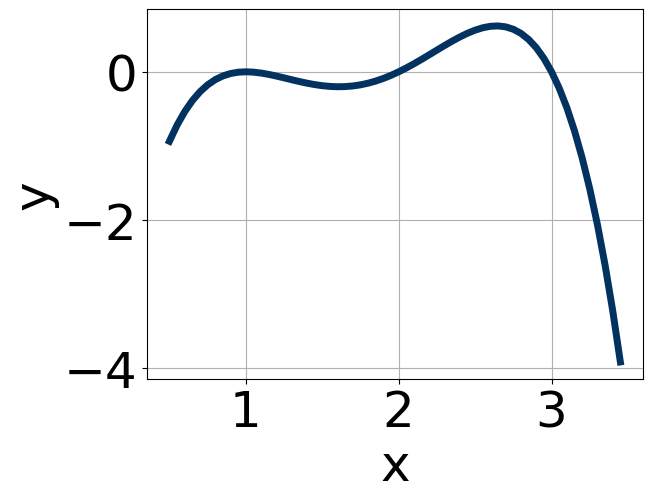
\includegraphics[width=0.5\textwidth]{../Figures/polyGraphToFunctionCopyB.png}
\end{center}


The solution is \( -8(x - 1)^{8} (x - 3)^{7} (x - 2)^{5} \).\begin{enumerate}[label=\Alph*.]
\textbf{Plausible alternative answers include:}* This is the correct option.
This corresponds to the leading coefficient being the opposite value than it should be.
The factor $1$ should have an even power and the factor $3$ should have an odd power.
The factor $(x - 3)$ should have an odd power.
The factor $(x - 2)$ should have an odd power and the leading coefficient should be the opposite sign.
\end{enumerate}

\textbf{General Comment:} General Comments: Draw the x-axis to determine which zeros are touching (and so have even multiplicity) or cross (and have odd multiplicity).
}
\litem{
Construct the lowest-degree polynomial given the zeros below.
\[ -2 + 2 i \text{ and } 3 \]The solution is \( x^{3} + x^{2} -4 x -24 \).\begin{enumerate}[label=\Alph*.]
\textbf{Plausible alternative answers include:}$x^{3} + x^{2} -x -6$, which corresponds to multiplying out $(x + 2)(x -3)$.
$x^{3} + x^{2} -5 x + 6$, which corresponds to multiplying out $(x -2)(x -3)$.
* $x^{3} + x^{2} -4 x -24$, which is the correct option.
$x^{3} -1 x^{2} -4 x + 24$, which corresponds to multiplying out $(x-(-2 + 2 i))(x-(-2 - 2 i))(x + 3)$.
This corresponds to making an unanticipated error or not understanding how to use nonreal complex numbers to create the lowest-degree polynomial. If you chose this and are not sure what you did wrong, please contact the coordinator for help.
\end{enumerate}

\textbf{General Comment:} Remember that the conjugate of $a+bi$ is $a-bi$. Since these zeros always come in pairs, we need to multiply out $(x-(-2 + 2 i))(x-(-2 - 2 i))(x-(3))$.
}
\litem{
Describe the end behavior of the polynomial below.
\[ f(x) = 5(x + 9)^{4}(x - 9)^{7}(x - 7)^{4}(x + 7)^{4} \]The solution is the graph below.
    \begin{center}
        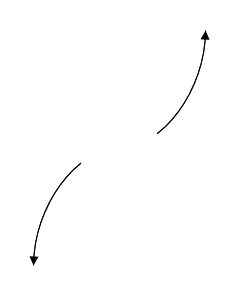
\includegraphics[width=0.3\textwidth]{../Figures/polyEndBehaviorDB.png}
    \end{center}

\textbf{General Comment:} Remember that end behavior is determined by the leading coefficient AND whether the \textbf{sum} of the multiplicities is positive or negative.
}
\end{enumerate}

\end{document}